\documentclass[11pt,a4paper]{article}
\usepackage[a4paper,top=13mm,bottom=13.5mm,left=14mm,right=14mm,headsep=5mm,footskip=6mm]{geometry}
\usepackage[T1]{fontenc}
\usepackage{libertinus}
\usepackage[final]{microtype}
\usepackage{amsmath,amssymb,mathtools,bm}
\usepackage{xcolor}
\usepackage{multicol,booktabs,tabularx,array,enumitem}
\usepackage{tikz}
\usetikzlibrary{arrows.meta,positioning,calc,decorations.pathreplacing}
\usepackage[most]{tcolorbox}
\usepackage{fancyhdr}
\usepackage{hyperref}
\hypersetup{colorlinks=true,linkcolor=teal!50!black,urlcolor=teal!45!black,pdftitle={PHYS7045: 2026 Assignment Formula and Methods Sheet},pdfauthor={PHYS7045 Exam Revision}}
\definecolor{ink}{HTML}{263746}
\definecolor{accent}{HTML}{11677A}
\definecolor{muted}{HTML}{586A78}
\definecolor{soft}{HTML}{F0F5F7}
\definecolor{warm}{HTML}{F9F6EE}
\AtBeginDocument{\color{ink}}
\setlength{\parindent}{0pt}
\setlength{\parskip}{2.3pt plus .5pt minus .4pt}
\setlength{\columnsep}{7mm}
\setlength{\columnseprule}{.2pt}
\setlength{\multicolsep}{2pt}
\setlength{\emergencystretch}{2.5em}
\setlist[enumerate]{leftmargin=*,topsep=1.5pt,itemsep=.8pt,parsep=0pt}
\setlist[itemize]{leftmargin=*,topsep=1.5pt,itemsep=.8pt,parsep=0pt}
\newcommand{\ket}[1]{\left\lvert #1\right\rangle}
\newcommand{\bra}[1]{\left\langle #1\right\rvert}
\newcommand{\braket}[2]{\left\langle #1\middle|#2\right\rangle}
\newcommand{\I}{\mathbb I}
\newcommand{\Tr}{\operatorname{Tr}}
\newcommand{\D}{\mathcal D}
\newcommand{\ee}{\mathrm e}
\newcommand{\wt}{\operatorname{wt}}
\newcommand{\smallbox}[1]{\begin{tcolorbox}[colback=soft,colframe=accent!40!white,boxrule=.4pt,arc=1mm,left=1.2mm,right=1.2mm,top=.65mm,bottom=.65mm,before skip=2pt,after skip=2pt]\footnotesize #1\end{tcolorbox}}
\newcommand{\caution}[1]{\begin{tcolorbox}[colback=warm,colframe=black!17,boxrule=.35pt,arc=1mm,left=1.2mm,right=1.2mm,top=.65mm,bottom=.65mm,before skip=2pt,after skip=2pt]\footnotesize #1\end{tcolorbox}}
\newcommand{\topic}[1]{\par\vspace{3pt}{\color{accent}\bfseries #1}\par\vspace{-1pt}}
\newcommand{\paper}[1]{{\color{muted}\footnotesize\emph{#1}}}
\newcommand{\pagetitle}[2]{\noindent{\color{accent}\fontsize{15.5}{18}\selectfont\bfseries #1}\hfill{\footnotesize\color{muted}#2}\par\vspace{1pt}\hrule\vspace{4pt}}
\pagestyle{fancy}
\fancyhf{}
\fancyhead[L]{\footnotesize\color{muted}PHYS7045 \textbar\ 2026 Assignment Methods}
\fancyhead[R]{\footnotesize\color{muted}Recognise \textrightarrow\ calculate \textrightarrow\ check}
\fancyfoot[L]{\scriptsize\color{muted}A1 quantum information \textbullet\ A2 noise/QEC \textbullet\ A3 hardware}
\fancyfoot[R]{\footnotesize\bfseries\color{accent}\thepage\ / 5}
\renewcommand{\headrulewidth}{.2pt}
\renewcommand{\footrulewidth}{0pt}
\begin{document}
\pagetitle{1. Assignment 1: states, rotations and control}{A1 Q1.1--Q1.2}
\begin{multicols}{2}\small
\topic{A. From a qubit ket to its Bloch vector}
\paper{Q1.1(a): prove the density-operator/Bloch relation.}
Write the state, form its outer product, then compare coefficients of the Pauli matrices:
\[\ket\psi=\cos\frac\theta2\ket0+\ee^{i\phi}\sin\frac\theta2\ket1,\]
\[\boxed{\rho=\ket\psi\bra\psi=\frac12(\I+\bm r\cdot\bm\sigma)},\qquad
\bm r=\begin{pmatrix}\sin\theta\cos\phi\\\sin\theta\sin\phi\\\cos\theta\end{pmatrix}.\]
\[\rho=\frac12\begin{pmatrix}1+r_z&r_x-ir_y\\r_x+ir_y&1-r_z\end{pmatrix},\quad
r_i=\Tr(\rho\sigma_i).\]
\textbf{How to prove:} use $\cos^2(\theta/2)=(1+\cos\theta)/2$ and $2\cos(\theta/2)\sin(\theta/2)=\sin\theta$. Pure states have $|\bm r|=1$; mixed qubits have $|\bm r|\le1$.

\topic{B. Pauli algebra and exponentiation}
\paper{Q1.1(b)--(c): the two standard proof shortcuts.}
\[\boxed{\sigma_i\sigma_j=\delta_{ij}\I+i\sum_k\epsilon_{ijk}\sigma_k},\quad
\{\sigma_i,\sigma_j\}=2\delta_{ij}\I.\]
For a \emph{unit} vector $\bm n$, $A=\bm n\cdot\bm\sigma$ satisfies $A^2=\I$. Separate even and odd terms of $\ee^{i\vartheta A}$:
\[\boxed{\ee^{\pm i\vartheta A}=\I\cos\vartheta\pm iA\sin\vartheta}.\]
\textbf{Approach:} check the square first; this works for a two-qubit Pauli product as well (e.g. $Y\otimes Y$).

\topic{C. Show a unitary really rotates the Bloch sphere}
\paper{Q1.1(d) and advanced general-axis rotation.}
\[\boxed{R_{\bm n}(\alpha)=\ee^{-i\alpha\bm n\cdot\bm\sigma/2}},\qquad
\rho'=R\rho R^\dagger.\]
Use $R\sigma_jR^\dagger$ and read off the new Bloch-vector coefficients. For example,
\[\begin{aligned}R_x:\ (r_x,r_y,r_z)\mapsto \big(&r_x,\ r_y\cos\alpha-r_z\sin\alpha,\\&r_y\sin\alpha+r_z\cos\alpha\big).\end{aligned}\]
The analogous cyclic expressions give $R_y,R_z$. General rotation is described by Rodrigues' formula:
\[\boxed{\bm r'=\bm r\cos\alpha+(\bm n\times\bm r)\sin\alpha+\bm n(\bm n\cdot\bm r)(1-\cos\alpha)}.\]
\caution{A positive sign in $\exp(+i\alpha\bm n\cdot\bm\sigma/2)$ gives the opposite active rotation under the convention $\rho'=R\rho R^\dagger$. State your sign convention.}

\columnbreak
\topic{D. Hamiltonian $\to$ rotation axis $\to$ pulse time}
\paper{Q1.2(a)--(c): recognise the $X$ and $Z$ controls.}
\[H=\hbar(t_cX+\Delta Z),\quad\omega=\sqrt{t_c^2+\Delta^2},\]
\[\boxed{U(\tau)=\cos(\omega\tau)\I-i\sin(\omega\tau)\frac{t_cX+\Delta Z}{\omega}}.\]
The Bloch rotation angle is $\alpha=2\omega\tau$. For $X_\alpha$, set $\Delta=0$; for $Z_\alpha$, set $t_c=0$. Hence
\[\boxed{\tau_X=\frac\alpha{2t_c},\qquad\tau_Z=\frac\alpha{2\Delta}}.\]
At the specified maxima $t_c/2\pi=5$ GHz and $\Delta/2\pi=40$ GHz,
\[\tau_{X_\pi}^{\min}=50\,\mathrm{ps},\qquad\tau_{Z_\pi}^{\min}=6.25\,\mathrm{ps}.\]
Use Euler decompositions for other axes, e.g.
\[R_y(\alpha)=R_z(\pi/2)R_x(\alpha)R_z(-\pi/2),\]
with matrix order as written (the rightmost pulse acts first). An explicit Hadamard synthesis, up to a global phase, is
\[\boxed{H\sim R_z(\pi/2)R_x(\pi/2)R_z(\pi/2)}.\]

\topic{E. Timing diagrams with 1 ns resolution}
\paper{Q1.2(d) and advanced conditional control.}
\begin{enumerate}
\item Rewrite every target gate as an ordered sequence of $X_\alpha$ and $Z_\alpha$ rotations; rightmost matrix acts first.
\item Choose an \emph{integer} number $m$ of 1 ns slots; set $t_c=\alpha/(2m\,\mathrm{ns})$ or $\Delta=\alpha/(2m\,\mathrm{ns})$ (if within the hardware bounds).
\item Draw horizontal levels for $t_c(t)$, $\Delta(t)$, and the interaction switch $C(t)$; label durations and accumulated angles.
\item At the measurement stage choose $t_c=0$, so a $Z$ Hamiltonian does not change computational-basis outcome probabilities.
\end{enumerate}
\smallbox{\textbf{Concrete pulse:} an $X_\pi$ rotation in one 1 ns step needs $t_c/(2\pi)=0.25$ GHz (not the 5 GHz maximum). The 1 ns clock constrains duration, not the available analogue amplitude.}

\topic{F. Conditional $ZZ$ phase and CNOT}
\paper{Q1.2 Part B: two control-state-dependent shifts.}
With interaction on ($C=1$) and $t_c=0$, the target has $Z$ rate $\Delta+\delta_{0,1}$ according to control $\ket0,\ket1$. Their \emph{difference} produces the entangling phase:
\[\boxed{\chi=2(\delta_1-\delta_0)\tau\pmod{2\pi}}.\]
For $\delta_1-\delta_0=2\pi\,50$ MHz, $\chi=\pi$ at $\tau=5$ ns. Correct the additional \emph{local} $Z$ phases to obtain CZ; then
\[\boxed{\mathrm{CNOT}=(\I\otimes H)\,\mathrm{CZ}\,(\I\otimes H)}.\]
\topic{G. No-cloning theorem in three lines}
\paper{Q1.1 Part B(b).}
Suppose a unitary clones $\ket u$ and $\ket v$. Inner products are preserved, but those of two copies square:
\[\braket uv=\braket uv^2\Rightarrow\braket uv\in\{0,1\}.\]
Nonorthogonal, distinct states violate this: \emph{linearity/unitarity forbids universal cloning}.
\end{multicols}
\clearpage
\pagetitle{2. Assignment 1: entanglement and fidelity}{A1 Q1.3--Q1.4}
\begin{multicols}{2}\small
\topic{A. Schmidt decomposition: how to find it}
\paper{Q1.3(a)--(d): pair orthonormal states across a bipartition.}
Given
\[\ket\Psi=\tfrac1{\sqrt2}(\ket{\alpha_1}_A\ket0_B+\ket{\alpha_2}_A\ket1_B),\]
\[\ket{\alpha_1}=\cos\theta\ket0+\sin\theta\ket1,\quad
\ket{\alpha_2}=\cos\theta\ket0-\sin\theta\ket1,\]
collect terms by Alice's computational basis and introduce $\ket\pm=(\ket0\pm\ket1)/\sqrt2$:
\[\boxed{\ket\Psi=\cos\theta\ket0_A\ket+_B+\sin\theta\ket1_A\ket-_B}.\]
Absorb any negative coefficient into its associated ket; the \emph{Schmidt coefficients} are $|\cos\theta|,|\sin\theta|$.

\textbf{General algorithm:} (1) write the amplitudes as a matrix $M_{ij}$; (2) find the singular-value decomposition $M=U\Sigma V^\dagger$; (3) squared singular values $\lambda_j$ are eigenvalues of $\rho_A$ and $\rho_B$. Schmidt bases are unique up to phases except within degenerate coefficients; zero-coefficient subspaces are unconstrained.

\topic{B. Partial trace and von Neumann entropy}
\[\rho_B=\Tr_A\ket\Psi\bra\Psi
=\cos^2\theta\ket+\bra++\sin^2\theta\ket-\bra-,\]
\[\boxed{\rho_B=\frac12\begin{pmatrix}1&\cos2\theta\\\cos2\theta&1\end{pmatrix}}.\]
\[\boxed{S(\rho_B)=-\sum_j\lambda_j\log_2\lambda_j},\qquad
\lambda_\pm=\cos^2\theta,\sin^2\theta.\]
\textbf{Check:} $S=0$ for product states; $S=1$ bit for $|\cos\theta|=|\sin\theta|$.

\topic{C. Unambiguous state discrimination (USD)}
\paper{Q1.3 advanced: use positivity and no signalling.}
The two possible Alice states overlap by
\[s=\braket{\alpha_1}{\alpha_2}=\cos 2\theta.\]
Let $p_1,p_2$ be success probabilities conditioned on the equiprobable states. Because Alice's local action cannot alter Bob's unconditional state, the unnormalised Bob ``failure'' operator must be positive:
\[\rho_B^{\rm fail}=\tfrac12\begin{pmatrix}1-p_1&s\\s&1-p_2\end{pmatrix}\succeq0.\]
Thus $(1-p_1)(1-p_2)\ge |s|^2$. By AM--GM,
\[\boxed{P_{\rm success}=\tfrac{p_1+p_2}2\le1-|s|=1-|\cos2\theta|}.\]
This is tight for equal priors. USD may have an inconclusive result but \emph{never} falsely identifies a state.

\columnbreak
\topic{D. Teleportation through a nonmaximal Bell pair}
\paper{Q1.4 Part A: calculate the output \emph{with outcome weights}.}
Input $\ket a=\alpha\ket0+\zeta\ket1$ with $\alpha=\cos(\theta/2)$, $\zeta=\ee^{i\phi}\sin(\theta/2)$. Resource:
\[\ket{AB}=\cos\beta\ket{01}-\sin\beta\ket{10}.\]
\textbf{Do this in order:}
\begin{enumerate}
\item Expand $\ket a\otimes\ket{AB}$ in the $(a,A,B)$ ordering.
\item Project Alice's two systems onto $\Phi^\pm=(\ket{00}\pm\ket{11})/\sqrt2$ and $\Psi^\pm=(\ket{01}\pm\ket{10})/\sqrt2$.
\item Apply Bob's outcome-specific Pauli correction. The \emph{unnormalised} corrected state for either $\Phi$ outcome is $\tfrac1{\sqrt2}(\alpha\cos\beta\ket0+\zeta\sin\beta\ket1)$; for either $\Psi$ outcome it is $\tfrac1{\sqrt2}(\alpha\sin\beta\ket0+\zeta\cos\beta\ket1)$, up to a global phase.
\item Sum corrected density operators, retaining outcome probabilities automatically.
\end{enumerate}
\[\boxed{\rho_{\rm out}=\begin{pmatrix}|\alpha|^2&\alpha\zeta^*\sin2\beta\\ \alpha^*\zeta\sin2\beta&|\zeta|^2\end{pmatrix}}.\]
This is a dephasing channel on the input Bloch sphere: $z$ population is preserved; transverse coherence is reduced by $\sin2\beta$.

\topic{E. Fidelity, then average over unknown inputs}
For a pure target and mixed output,
\[F=\bra a\rho_{\rm out}\ket a.
\]
Substitute $\alpha,\zeta$:
\[\boxed{F(\theta,\phi)=1-\tfrac12(1-\sin2\beta)\sin^2\theta}.\]
There is no $\phi$ dependence. Uniform Bloch-sphere averaging uses the \emph{area element} $\sin\theta\,d\theta\,d\phi$:
\[\bar F=\frac1{4\pi}\int_0^{2\pi}\!\int_0^\pi F\sin\theta\,d\theta\,d\phi,\]
\[\boxed{\bar F=\frac{2+\sin2\beta}{3}}.\]
\textbf{Checks:} $\beta=\pi/4\Rightarrow F=1$; $\beta=0\Rightarrow \bar F=2/3$, the classical limit for an unknown qubit.

\topic{F. Werner-state teleportation}
\paper{Q1.4 Part B: exploit linearity instead of redoing Bell projections.}
\[\rho_W=(1-p)\ket{\Psi^-}\bra{\Psi^-}+\tfrac p4\I_4.\]
The Bell resource teleports perfectly; the fully mixed part produces $\I_2/2$. Therefore
\[\boxed{\rho_{\rm out}=(1-p)\ket a\bra a+\frac p2\I_2,\quad F=1-\frac p2}.\]
\smallbox{\textbf{Exam habit:} distinguish a \emph{conditional normalised} output (one measurement result) from the \emph{average} teleported state (sum over all four results). The latter is used for the usual fidelity.}
\end{multicols}
\clearpage
\pagetitle{3. Assignment 2: open systems and QEC}{A2 Q1--Q2}
\begin{multicols}{2}\small
\topic{A. Lindblad equation $\to$ Bloch differential equations}
\paper{Q1 Part A: arbitrary initial state, steady state, plots, purity.}
\[\dot\rho=-\frac{i\Omega}{2}[X,\rho]+\gamma\D[Z]\rho,\quad
\D[L]\rho=L\rho L^\dagger-\frac12\{L^\dagger L,\rho\}.\]
Insert $\rho=(\I+xX+yY+zZ)/2$. Compare the $X,Y,Z$ coefficients (or use $\dot r_j=\Tr(\sigma_j\dot\rho)$):
\[\boxed{\dot x=-2\gamma x,\quad\dot y=-2\gamma y-\Omega z,\quad\dot z=\Omega y}.\]
For $\Omega>\gamma>0$, let $\omega=\sqrt{\Omega^2-\gamma^2}$. With $(x_0,y_0,z_0)$ arbitrary,
\[\begin{aligned}
 x(t)&=x_0\ee^{-2\gamma t},\\[-1mm]
 y(t)&=\ee^{-\gamma t}\!\left[y_0\cos\omega t-\frac{\gamma y_0+\Omega z_0}{\omega}\sin\omega t\right],\\[-1mm]
 z(t)&=\ee^{-\gamma t}\!\left[z_0\cos\omega t+\frac{\gamma z_0+\Omega y_0}{\omega}\sin\omega t\right].
\end{aligned}\]
\textbf{Workflow:} derive ODEs $\to$ solve $\dot{\bm r}=A\bm r$ $\to$ set $\dot{\bm r}=0$ $\to$ recover $\rho(t)$ $\to$ plot $\bm r(t)$ and purity:
\[\rho_{\rm ss}=\I/2\quad(\Omega,\gamma>0),\qquad\boxed{\Tr\rho^2=\frac{1+x^2+y^2+z^2}{2}}.\]
For $\ket0$ initially, $(x_0,y_0,z_0)=(0,0,1)$. If $\Omega\le\gamma$, use real exponential/hyperbolic solutions instead of oscillatory sines. Pure dephasing with $\Omega=0$ leaves $z$ conserved.

\topic{B. Damped atom $\to$ Kraus representation}
\paper{Q1 Part B: generalized amplitude damping.}
For $\ket g=(1,0)^T,\ket e=(0,1)^T$ define
\[\Gamma_\downarrow=\tfrac\gamma2(n+1),\quad \Gamma_\uparrow=\tfrac\gamma2 n,\quad \Gamma_1=\tfrac\gamma2(2n+1).\]
Then $x,y\propto \ee^{-\Gamma_1t/2}$ and
\[\boxed{z(t)=z_\infty+(z_0-z_\infty)\ee^{-\Gamma_1t},\quad z_\infty=\frac1{2n+1}}.\]
Set $q=(n+1)/(2n+1)$ (ground equilibrium probability), $\lambda=1-\ee^{-\Gamma_1t}$:
\[\begin{array}{@{}ll@{}}
K_0=\sqrt q\begin{pmatrix}1&0\\0&\sqrt{1-\lambda}\end{pmatrix},&
K_1=\sqrt q\begin{pmatrix}0&\sqrt\lambda\\0&0\end{pmatrix},\\[2mm]
K_2=\sqrt{1-q}\begin{pmatrix}\sqrt{1-\lambda}&0\\0&1\end{pmatrix},&
K_3=\sqrt{1-q}\begin{pmatrix}0&0\\\sqrt\lambda&0\end{pmatrix}.
\end{array}\]
Check $\sum_jK_j^\dagger K_j=\I$, $t=0$ gives identity and $t\to\infty$ gives thermal equilibrium.

\columnbreak
\topic{C. The Steane code: start with the parity checks}
\paper{Q2 Part A: Tanner graph, logicals, distance, syndromes.}
\[\boxed{[[n,k,d]]=[[7,1,3]],\qquad k=n-r=7-6=1.}\]
The three $X$-check supports are $\{4,5,6,7\}$, $\{2,3,6,7\}$, $\{1,3,5,7\}$; the $Z$ checks have the same supports. The classical parity-check matrix is
\[H=\begin{pmatrix}0&0&0&1&1&1&1\\0&1&1&0&0&1&1\\1&0&1&0&1&0&1\end{pmatrix}.\]
\textbf{Tanner graph:} draw one vertex for each physical qubit, another for each parity check, and an edge wherever $H_{ij}=1$.

All same-Pauli checks commute. Opposite-type checks overlap in $4$ (same support) or $2$ (different supports) locations, hence an \emph{even} number of $XZ$ anticommutations, so they commute.

\topic{D. General syndrome-lookup algorithm}
The syndrome of $X_j$ is the $j$th column of $H$, measured by the \emph{$Z$ checks}; swap roles for $Z_j$:
\[\begin{array}{@{}c|cccccccc@{}}\text{syndrome}&000&001&010&011&100&101&110&111\\\hline
\text{qubit}&--&1&2&3&4&5&6&7\end{array}\]
\textbf{Steps:} measure three $Z$ checks $\to$ correct $X_j$; measure three $X$ checks $\to$ correct $Z_k$. A $Y_j=iX_jZ_j$ generates \emph{both} signatures. The syndrome measures an error without observing logical amplitudes.

Logical representatives $X_L=X^{\otimes7}$, $Z_L=Z^{\otimes7}$ commute with all checks and anticommute with each other. Multiply by stabilisers:
\[X_L(\I\I\I X X X X)=X_1X_2X_3,\]
\[Z_L(\I\I\I Z Z Z Z)=Z_1Z_2Z_3.\]
Thus $d\le3$, while distinct nonzero single-error syndromes rule out nontrivial weight-$1$ or weight-$2$ logicals; hence $d=3$.

\topic{E. Failure probability and transversal CNOT}
\paper{Q2 Part A(4)--(5), Part B(a)--(b).}
For a bit-only independent-error rate $p$, an \emph{upper bound} follows from requiring at most one error:
\[\boxed{P_{\rm fail}\le1-(1-p)^7-7p(1-p)^6}.\]
The exact lookup decoder failure probability is
\[\boxed{\begin{aligned}P_{\rm fail}={}&21p^2(1-p)^5+7p^3(1-p)^4\\&+28p^4(1-p)^3+7p^6(1-p)+p^7.\end{aligned}}\]
For independent $X,Z$ sectors, sum sector-wise upper bounds (or use independence to bound by $1-P_{\le1}(p_X)P_{\le1}(p_Z)$). For a transversal logical CNOT, apply seven physical $\mathrm{CNOT}_{c_j\to t_j}$ gates and check Heisenberg transformations:
\[\boxed{X_L^c\mapsto X_L^cX_L^t,\qquad Z_L^t\mapsto Z_L^cZ_L^t},\]
with $Z_L^c,X_L^t$ unchanged.
\end{multicols}
\clearpage
\pagetitle{4. Assignment 3: blockade and ion pulses}{A3 Q1--Q2}
\begin{multicols}{2}\small
\topic{A. Rydberg blockade $\to$ controlled $X$ rotation}
\paper{Q1.1--Q1.5: control on $\ket0$, not $\ket1$.}
Here $\ket0\equiv\ket g$, $\ket1\equiv\ket r$, and the target is driven resonantly with angular Rabi frequency $\Omega$. If control is $\ket0$, the target rotates; if control is already $\ket r$, double excitation is off resonance:
\[U_x(\theta)=\ee^{-i\theta X/2}
=\begin{pmatrix}c&-is\\-is&c\end{pmatrix},\quad c=\cos\frac\theta2,\ s=\sin\frac\theta2.\]
\[\boxed{CU_x(\theta)=\begin{pmatrix}
 c&-is&0&0\\-is&c&0&0\\0&0&1&0\\0&0&0&1
\end{pmatrix}},\]
with ordered basis $\ket{00},\ket{01},\ket{10},\ket{11}$ (control first). Here $\theta=\Omega\tau$.

\textbf{Physical sequence:} initialise neighbouring atoms; shine the resonant laser at the target for $\tau$; in the $\ket{0}_c$ sector it performs Rabi oscillations, whereas in the $\ket{1}_c$ sector the interaction shifts $\ket{rr}$ and suppresses the target excitation.

\begin{center}
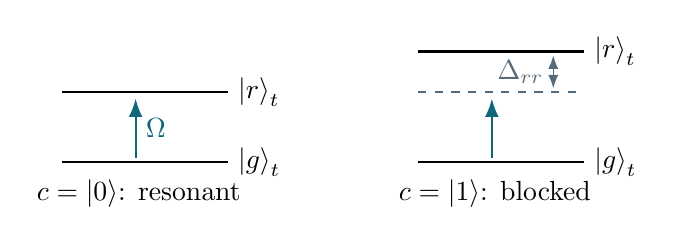
\begin{tikzpicture}[x=0.78cm,y=0.52cm,>=Latex]
\draw[thick] (0,0)--(2.7,0) node[right] {$\ket{g}_t$};
\draw[thick] (0,1.7)--(2.7,1.7) node[right] {$\ket{r}_t$};
\draw[->,thick,accent] (1.2,.1)--(1.2,1.55) node[midway,right] {$\Omega$};
\node[below] at (1.25,-.2) {$c=\ket0$: resonant};
\begin{scope}[shift={(5.8,0)}]
\draw[thick] (0,0)--(2.7,0) node[right] {$\ket{g}_t$};
\draw[thick,dashed,muted] (0,1.7)--(2.7,1.7);
\draw[thick] (0,2.7)--(2.7,2.7) node[right] {$\ket{r}_t$};
\draw[<->,muted] (2.2,1.8)--(2.2,2.6) node[midway,left] {$\Delta_{rr}$};
\draw[->,thick,accent] (1.2,.1)--(1.2,1.55);
\node[below] at (1.25,-.2) {$c=\ket1$: blocked};
\end{scope}
\end{tikzpicture}
\end{center}
The high-fidelity requirement is $|\Delta_{rr}|\gg\Omega$ if both are angular frequencies (or $|U_{rr}|\gg\hbar\Omega$ in energy units). Scalability is limited by finite-range blockade, crosstalk and Rydberg decay.

\topic{B. Turn $CU_x$ into an exact controlled NOT}
\paper{Q1.6--Q1.7: conditional phase matters.}
Choosing $\theta=3\pi$ yields $U_x(3\pi)=iX$, hence the control-$0$ sector picks up a relative phase $i$. Prepend $R_z(\pi/2)$ on the \emph{control}:
\[\boxed{CU_x(3\pi)\,[R_z(\pi/2)\otimes\I]
=\ee^{i\pi/4}\,C_0X},\]
where $C_0X$ flips the target only if control is $\ket0$. Conjugate with an $X$ on the control to obtain standard control-on-$1$ CNOT.
\[\boxed{\tau=\frac{3\pi}{\Omega};\qquad \frac\Omega{2\pi}=2\,\mathrm{kHz}\Rightarrow\tau=0.75\,\mathrm{ms}.}\]
\caution{A $\pi$ target pulse gives $-iX$, \emph{not} $X$. Its phase is conditional and requires local correction. Always distinguish pulse \emph{area} $\theta$ from duration $\tau$.}

\columnbreak
\topic{C. Trapped-ion sidebands: track motion explicitly}
\paper{Q2 Part A: $\pi_A,2\pi_B,\pi_A$ gate.}
Use $\ket{A\,B,n}$ with internal $g/e$ and shared phonon number $n$. A red sideband couples
\[\boxed{\ket{e,n}\leftrightarrow\ket{g,n+1}},\]
with a $\pi$ pulse contributing $-i$ each way, while $\ket{g,0}$ is dark. On ion B the auxiliary transition is $\ket{g,1}\leftrightarrow\ket{a,0}$: a $2\pi$ pulse returns it with sign $-1$.

\begin{center}\footnotesize
\renewcommand{\arraystretch}{1.15}
\begin{tabular}{@{}llll@{}}\toprule
Input&after $\pi_A$&after $2\pi_B$&after $\pi_A$\\\midrule
$\ket{gg,0}$&$\ket{gg,0}$&$\ket{gg,0}$&$\ket{gg,0}$\\
$\ket{ge,0}$&$\ket{ge,0}$&$\ket{ge,0}$&$\ket{ge,0}$\\
$\ket{eg,0}$&$-i\ket{gg,1}$&$+i\ket{gg,1}$&$+\ket{eg,0}$\\
$\ket{ee,0}$&$-i\ket{ge,1}$&$-i\ket{ge,1}$&$-\ket{ee,0}$\\\bottomrule
\end{tabular}
\end{center}
\[\boxed{U_{AB}=\operatorname{diag}(1,1,1,-1)=CZ}.\]
\textbf{Method:} write the effect of \emph{each} pulse on each basis input, include the phonon and phase, and only then build the $4\times4$ matrix. The shared mode must end in $\ket{0}$.

\topic{D. From CZ to CNOT; from CZ to CCZ}
\[\boxed{\mathrm{CNOT}_{A\to B}=(\I\otimes H)CZ(\I\otimes H)}.\]
For three ions $A,B,C$, add a red-sideband $\pi$ pulse to map the excitation of a second control (e.g. ion C) into the motional bus, then the auxiliary $2\pi$ conditional phase, then undo the mappings in reverse. The five-pulse pattern is schematically
\[\pi_A\;\pi_C\;2\pi_B\;\pi_C\;\pi_A.\]
With appropriate sideband addressing and phase conventions, only $\ket{eee}$ acquires a negative sign:
\[\boxed{CCZ=\operatorname{diag}(1,1,1,1,1,1,1,-1)}.\]
Conjugate by $H$ on target $B$ to obtain the Toffoli (CCNOT). The exact pulse design must ensure the bus distinguishes the intended control sector and returns to $n=0$.

\topic{E. Generic hardware-gate answer template}
\begin{enumerate}
\item Declare computational basis and any auxiliary states/modes.
\item Specify the resonant/detuned transition and why it is driven or dark.
\item Translate pulse area $\Theta=\Omega_{\rm eff}\tau$ into $-i$ for $\pi$ and $-1$ for $2\pi$ within the coupled two-state subspace.
\item Track relative phases; confirm all population returns to the computational manifold.
\item Build the gate and state necessary single-qubit corrections.
\end{enumerate}
\end{multicols}
\clearpage
\pagetitle{5. Assignment 3: circuits, photons and lookup}{A3 Q3--Q4 + complete index}
\begin{multicols}{2}\small
\topic{A. Cooper-pair box: start with $\mathcal L=T-V$}
\paper{Q3.1--Q3.4: derive instead of guessing the Hamiltonian.}
Node flux $\Phi$ is the generalised coordinate, with voltage $\dot\Phi$. The Josephson potential is $-E_J\cos\varphi$, where $\varphi=2\pi\Phi/\Phi_0$ and $\Phi_0=h/(2e)$. With $C_\Sigma=C_0+C_c$,
\[\boxed{\mathcal L=\tfrac12C_0\dot\Phi^2+\tfrac12C_c(\dot\Phi-V_g)^2+E_J\cos\varphi}.\]
\textbf{Standard four-step method:}
\begin{enumerate}
\item Compute conjugate charge: $Q=\partial\mathcal L/\partial\dot\Phi=C_\Sigma\dot\Phi-C_cV_g$.
\item Solve $\dot\Phi=(Q+C_cV_g)/C_\Sigma$.
\item Legendre transform $H=Q\dot\Phi-\mathcal L$, dropping only terms constant in $Q,\Phi$:
\[\boxed{H=\frac{(Q+C_cV_g)^2}{2C_\Sigma}-E_J\cos\varphi}.\]
\item Quantise $[\Phi,Q]=i\hbar$, then write $H\psi=E\psi$ (in flux representation, $Q=-i\hbar\partial_\Phi$).
\end{enumerate}
For $V_g=0$ near a Josephson minimum, $\cos\varphi\simeq1-\varphi^2/2$ and
\[\boxed{\hbar\omega_p=\sqrt{8E_JE_C},\qquad E_C=\frac{e^2}{2C_\Sigma}},\]\[\boxed{E_m\simeq-E_J+\hbar\omega_p\left(m+\tfrac12\right)}.\]
Therefore $E_1-E_0\simeq\sqrt{8E_JE_C}$. The nonquadratic cosine produces weak anharmonicity (the resource for selectively addressing the $\ket0\to\ket1$ transition).

\topic{B. Numerical spectrum: charge-basis matrix}
\paper{Q3.5--Q3.6: truncate and diagonalise.}
Define $n=Q/(2e)$ and $n_g=-C_cV_g/(2e)$. Then
\[\boxed{H=4E_C(n-n_g)^2-E_J\cos\varphi}.\]
In the integer Cooper-pair basis, $\ee^{\pm i\varphi}\ket n=\ket{n\pm1}$, giving the tridiagonal matrix
\[\boxed{H_{nm}=4E_C(n-n_g)^2\delta_{nm}-\frac{E_J}{2}(\delta_{n,m+1}+\delta_{n,m-1})}.\]
\textbf{Approach:} choose symmetric cutoff $n=-N,\dots,N$; compute lowest four eigenvalues vs $n_g$; increase $N$ until results converge; minimise $E_1(n_g)-E_0(n_g)$ over one period ($n_g\in[0,1]$). The smallest gap is near half-integer offset charge (the charge-degeneracy point). For an exact numerical value use the specified capacitance and $E_J$ ratios, not the harmonic approximation.

\columnbreak
\topic{C. Beam splitters, Bell states, HOM and MZI}
\paper{Q4 Part A/B: transform \emph{creation operators} rather than guessing photon paths.}
Choose one balanced-beam-splitter convention and use it consistently for both polarisations:
\[a_s^\dagger\mapsto\frac{c_s^\dagger+d_s^\dagger}{\sqrt2},\quad b_s^\dagger\mapsto\frac{c_s^\dagger-d_s^\dagger}{\sqrt2},\qquad s=H,V.\]
\textbf{Calculation algorithm:} (1) rewrite a Bell ket using $a_H^\dagger a_V^\dagger\ket{\mathrm{vac}}$ etc.; (2) replace the operators with their outputs; (3) commute bosonic operators; (4) convert $(c^\dagger)^2\ket{\rm vac}=\sqrt2\ket2$; (5) group and normalise output states.

For the \emph{antisymmetric} singlet input,
\[\boxed{\ket{\Psi^-}_{ab}=\frac{a_H^\dagger b_V^\dagger-a_V^\dagger b_H^\dagger}{\sqrt2}\ket{\rm vac}},\]
all bunched terms cancel, giving a coincidence of one photon per output port (up to an overall phase):
\[\ket{\Psi^-}_{ab}\to-\ket{\Psi^-}_{cd}.\]
For symmetric inputs $\ket{\Psi^+},\ket{\Phi^\pm}$, coincidence terms cancel and photons bunch; the $H/V$ content of the bunch differs between Bell states. For instance, with our convention,
\[\boxed{\ket{\Psi^+}\to\frac{\ket{HV,0}-\ket{0,HV}}{\sqrt2}}.\]
The relative sign depends on the beam-splitter convention and which input/output ports are labelled $a,b,c,d$.

In a balanced Mach--Zehnder interferometer, both arms undergo another common-mode optical unitary. The singlet's antisymmetric structure is invariant up to phase, so it still gives one count at each output detector. This is \emph{HOM-type two-photon interference} (antibunching of the antisymmetric state), not ordinary HOM bunching. A coincidence alone does not prove indistinguishability: vary arrival-time delay experimentally.

\topic{D. Five-page map of \emph{every assignment}}
\begin{center}\footnotesize
\begin{tabularx}{\linewidth}{@{}p{22mm}Xc@{}}\toprule
Question&Method to locate&Page\\\midrule
A1 Q1.1&Bloch, Pauli, rotations; no cloning&1\\
A1 Q1.2&Pulse amplitude, timing, controlled phase&1\\
A1 Q1.3&Schmidt, trace, entropy, USD bound&2\\
A1 Q1.4&Bell projection, fidelity, Werner state&2\\
A2 Q1&Bloch ODEs, steady state, thermal Kraus&3\\
A2 Q2&Steane Tanner graph, lookup, failure, CNOT&3\\
A3 Q1&Blockade, controlled $U_x$, pulse phase&4\\
A3 Q2&Red-sideband pulses, CZ and CCZ&4\\
A3 Q3&CPB Lagrangian, spectrum, gap&5\\
A3 Q4&Bell-state optics, MZI, HOM&5\\\bottomrule
\end{tabularx}
\end{center}
\caution{\textbf{Last check:} specify basis and ordering; distinguish angular $\Omega$ from $\Omega/(2\pi)$; keep conditional phases; include phonon numbers; normalise Fock states; test $\Tr\rho=1$, $\sum K_j^\dagger K_j=\I$ and $U^\dagger U=\I$. For full derivations use the three submitted assignment solution PDFs.}
\end{multicols}
\end{document}